
\section{External evaluation audit}
The post-hoc matched-FPR and precision--recall summaries use target labels. The two-sided exact Wilcoxon signed-rank sensitivity test for the 13 ImpactMesh AP differences gives $p=0.00049$.

Fig.~\ref{fig:external_review_events} plots the AP increment against ordinary self-training's miss rate and reference floodwater prevalence. Some high-miss ImpactMesh floods had large gains. EMSR799 missed all reference floodwater under ordinary self-training and still gained only 1.40 AP points, illustrating the spread at similar miss rates.

\begin{figure}[pos=H]
\centering
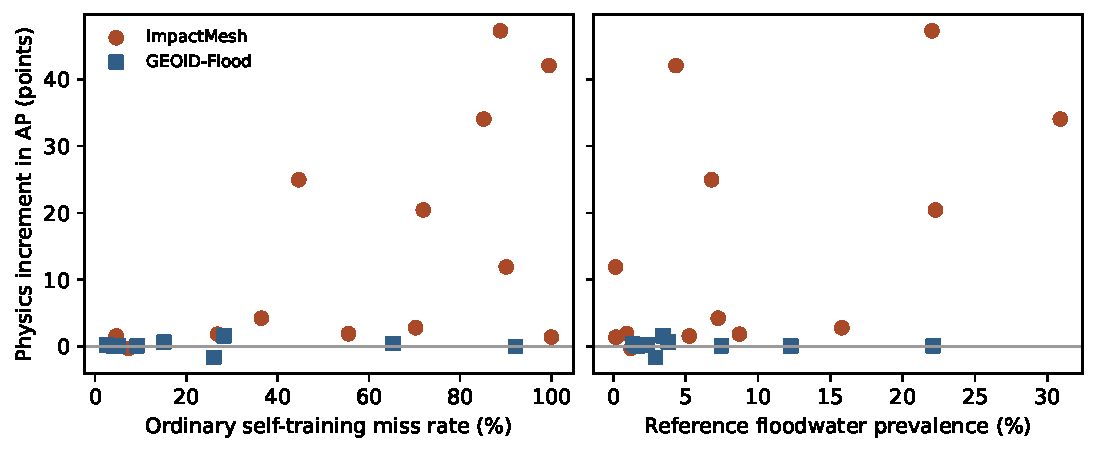
\includegraphics[width=\textwidth]{figures/fig_external_review_events.pdf}
\caption{Exploratory event-level associations across 22 activations. Miss rates use each cohort's source threshold. Prevalence is the share of scored pixels labelled as floodwater. AP differences compare physics-guided and ordinary self-training within an activation.}
\label{fig:external_review_events}
\end{figure}

Fig.~\ref{fig:external_review_pr} shows higher mean precision for physics-guided self-training at most recall levels on single-date ImpactMesh. On GEOID-Flood the two curves nearly overlap, consistent with the small AP difference between the two self-training arms.

\begin{figure}[pos=H]
\centering
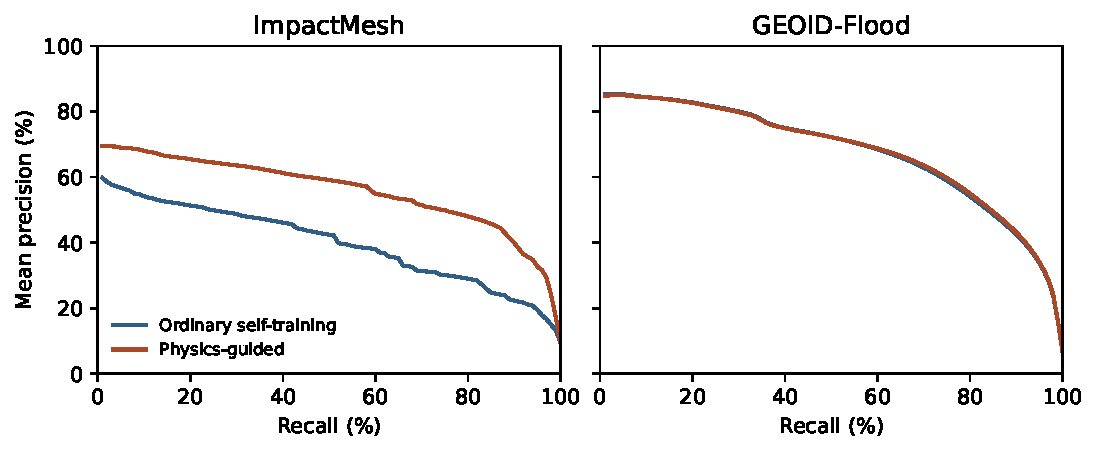
\includegraphics[width=\textwidth]{figures/fig_external_review_pr.pdf}
\caption{Macro precision--recall curves for the two self-training arms, computed at common recall levels from 1,000-bin score histograms. At each recall level we select the highest threshold reaching that recall in each activation and seed, and average precision across seeds and then activations. AP in the main comparison uses the original unrounded scores.}
\label{fig:external_review_pr}
\end{figure}

Fig.~\ref{fig:impactmesh_review_targets} shows the targets the rule would add to the initial teacher on the EMSR795 example. The rule selects both reference-flood and reference-dry pixels, illustrating how added supervision can recover floodwater and introduce false alarms.

\begin{figure}[pos=H]
\centering
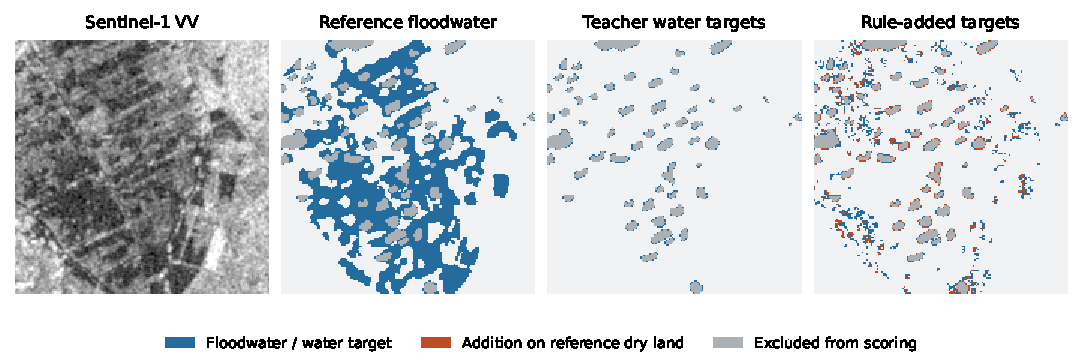
\includegraphics[width=\textwidth]{figures/fig_impactmesh_review_targets.pdf}
\caption{Illustration of the label additions on the EMSR795 chip from the main text. We apply the rule to the initial, AdaBN-adapted teacher's probabilities on the full chip (seed 0). The last panel marks pixels the rule would newly label as water, including 1,676 reference-flood and 1,960 reference-dry pixels. Reference labels colour these additions after inference. This full-chip snapshot is separate from the random training crops and their evolving teacher.}
\label{fig:impactmesh_review_targets}
\end{figure}

For GEOID-Flood, the first three archived protocol revisions resolved the publisher's activation coverage and accepted sub-micrometre rounding in otherwise coincident grids. The final version checks identical dimensions and coordinate reference systems with $10^{-6}$\,m absolute tolerances for nominal pixel sizes and companion-grid corner differences. These fixes preceded outcome scoring and required no resampling. The registered test and the established nine-activation coverage are documented alongside the immutable protocol archives.

The post-hoc GEOID-Flood radar-only controls use the same archived chip windows and class support. Before scoring, we verified the source shard checksums, all 708 selected radar and label raster digests, and the reference floodwater and dry-pixel counts for every activation.

For ImpactMesh, the local snapshot used to produce the scores has SHA-256 prefix \texttt{622bd37f8c5beb55}. The complete digest is recorded in the archived checksum file. The snapshot records the cohort, code, checkpoints, input hashes and analysis settings. Saved labels and 3,096 score arrays were hash-checked. Recalculation recovered every stored flood--seed AP and contingency count. Table~\ref{tab:impactmesh_lag} reports acquisition lag as a descriptive measure relative to Copernicus activation time.

To construct the matched-FPR curves for source, AdaBN and post-processing, we regenerated their control scores from the archived checkpoints and chips. The regenerated outputs reproduced the archived fixed-threshold contingency counts for all 117 controls. Of these, 90 reproduced the archived score digest exactly. The maximum absolute AP difference across all controls was $5.5\times10^{-11}$. For the 27 outputs with differing digests, a second CPU run at a different thread count reproduced all 54 matched-recall values exactly.

\begin{table}[pos=H]
\centering
\caption{ImpactMesh per-flood changes (physics-guided minus ordinary self-training, percentage points) and radar acquisition timing relative to activation. Miss and FPR differences use threshold 0.430. Lags describe the retained chips.}
\label{tab:impactmesh_lag}
\begin{tabular}{@{}lrrrrrrrr@{}}
\toprule
Activation & Chips & Flood (\%) & $\Delta$AP & $\Delta$Miss & $\Delta$FPR & Min d & Median d & Max d \\
\midrule
EMSR788 & 48 & 5.24 & +1.56 & -2.38 & +0.60 & 1.02 & 4.53 & 4.53 \\
EMSR789 & 48 & 8.71 & +1.84 & -15.95 & +2.99 & -2.21 & -2.21 & -2.21 \\
EMSR795 & 48 & 4.32 & +42.04 & -81.41 & +4.50 & 2.56 & 2.56 & 2.56 \\
EMSR797 & 15 & 1.21 & -0.29 & -0.86 & +0.25 & 1.07 & 1.07 & 1.07 \\
EMSR799 & 48 & 0.17 & +1.40 & -59.03 & +25.18 & 2.95 & 3.95 & 4.49 \\
EMSR802 & 48 & 6.78 & +24.96 & -39.97 & +1.63 & 0.47 & 0.47 & 0.47 \\
EMSR838 & 48 & 30.90 & +34.05 & -69.86 & +11.13 & -1.94 & -1.44 & 3.56 \\
EMSR843 & 13 & 0.15 & +11.90 & -18.30 & +0.09 & 1.62 & 1.62 & 1.62 \\
EMSR845 & 32 & 22.26 & +20.44 & -32.74 & +1.01 & -2.44 & -2.44 & -2.44 \\
EMSR848 & 48 & 22.02 & +47.26 & -58.82 & +1.63 & -3.25 & 21.74 & 22.26 \\
EMSR850 & 39 & 7.24 & +4.24 & -11.44 & +0.89 & 3.50 & 4.99 & 4.99 \\
EMSR851 & 33 & 15.79 & +2.80 & -8.69 & +0.88 & 0.42 & 0.42 & 6.94 \\
EMSR853 & 48 & 0.92 & +1.90 & -6.14 & +0.31 & 2.31 & 2.31 & 2.31 \\
\bottomrule

\end{tabular}
\end{table}

\begin{table}[pos=H]
\caption{GEOID-Flood paired changes in percentage points after averaging seeds within each activation. The primary comparison is the AP change from same-rule post-processing to physics-guided self-training. The remaining columns compare physics-guided with ordinary self-training. IoU, miss and FPR use the 0.208 source threshold.}
\label{tab:geoid_events}
\centering
\begin{tabular}{@{}lrrrrr@{}}
\toprule
 & vs. post-processing & \multicolumn{4}{c}{vs. ordinary self-training} \\
\cmidrule(lr){2-2}\cmidrule(lr){3-6}
Activation & $\Delta$AP & $\Delta$AP & $\Delta$IoU & $\Delta$Miss & $\Delta$FPR \\
\midrule
EMSR857 & +1.00 & +0.09 & -0.02 & -0.02 & +0.02 \\
EMSR858 & -0.48 & +0.01 & +0.45 & -1.09 & +0.09 \\
EMSR861 & +11.02 & +0.22 & -4.37 & -0.65 & +0.62 \\
EMSR864 & +1.48 & +0.07 & -0.79 & -0.43 & +0.30 \\
EMSR865 & +4.13 & +0.11 & -0.32 & -0.16 & +0.18 \\
EMSR866 & +4.81 & +1.59 & -2.38 & -4.36 & +0.76 \\
EMSR868 & +4.44 & +0.65 & -0.67 & -3.41 & +0.26 \\
EMSR870 & +4.08 & -1.65 & -4.12 & -1.53 & +0.59 \\
EMSR871 & +0.99 & +0.42 & -0.37 & -0.15 & +0.06 \\
\bottomrule

\end{tabular}
\end{table}


\subsection{Sensitivity to acquisition timing}
\label{sec:acquisition_timing}
At the chip level, restricting to radar acquisitions within three days either side of activation yielded a mean gain of 16.30 AP points, a median of 9.76, and gains on 11 of 12 scorable activations. Excluding EMSR848 as well yielded 13.68 mean points, 7.63 median points, and gains on 10 of 11 activations. A filter applied to each activation's median lag instead retained nine activations, already excluding EMSR848, with a mean gain of 15.51 points, median 11.90 and eight wins. These post-hoc analyses check sensitivity to activation timing. Activation time is an administrative timestamp.


\subsection{Exploratory label-free diagnostics}
Across the 22 external activations, the share of radar-valid pixels passing the two darkness thresholds had a Spearman correlation with AP gain of $0.26$ within ImpactMesh and $-0.57$ within GEOID-Flood (Fig.~\ref{fig:label_free_diagnostic}). On the 13 ImpactMesh activations, the rule candidate share assigned confidently dry by the initial teacher had a correlation of $0.51$. These post-hoc associations use fixed cue and teacher thresholds. The opposite signs for darkness coverage limit its use as a cross-cohort predictor, and the teacher-disagreement result is specific to ImpactMesh.

\begin{figure}[pos=t]
\centering
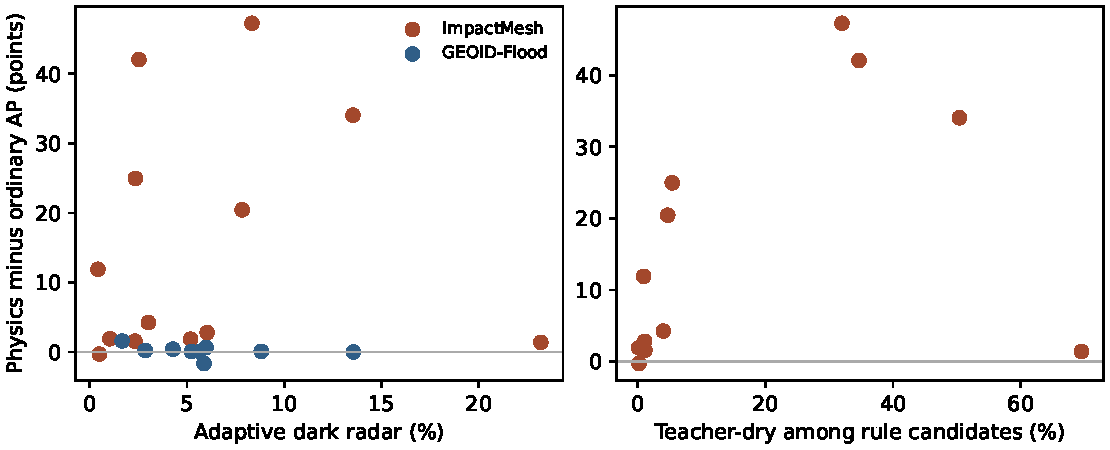
\includegraphics[width=\textwidth]{figures/exploratory_headroom.pdf}
\caption{Exploratory diagnostics based on radar inputs and initial teacher scores. Each point is one activation. The left panel shows the share of radar-valid pixels passing both adaptive darkness thresholds across the two external cohorts. For ImpactMesh, the right panel shows the share of terrain-gated rule candidates assigned dry with probability above 0.9 by the initial AdaBN teacher, averaged over three seeds. Only the AP difference on the vertical axis uses reference labels.}
\label{fig:label_free_diagnostic}
\end{figure}

\subsection{Practical note on normalisation for tiled SAR inference}
Prediction-time normalisation can depend on batch size \citep{nado2020predictionbn}. On the 26 Kuro Siwo development events, switching frozen weights from source running statistics to one-chip batch statistics reduced mean all-water AP from 76.26\% to 46.78\%. The paired mean difference was $-29.48$ points (95\% paired bootstrap interval $[-38.68,-20.32]$), with decreases on 23 of 26 events. Four-chip inference reached 77.18\% AP, and event re-estimation without gradient updates reached 83.75\%.


With Tent-adapted weights, event statistics gave 82.95\% AP and one-chip statistics gave 44.04\% (Table~\ref{tab:norm_external}). With weights fixed, four-chip inference recovered much of the lost AP. Its IoU remained lower than with source or event statistics at the same nominal miss target.

\begin{table}[pos=t]
\caption{Controlled Kuro Siwo normalisation experiment on 26 development events, using all-water support and three seeds. The weights and inference statistics vary as shown. AP is computed from 1,000 score bins. IoU, realised miss and FPR use leave-one-event-out (LOEO) thresholds at the nominal 20\% mean miss target.}
\label{tab:norm_external}
\centering
\begin{tabular}{@{}llrrrr@{}}
\toprule
Weights & Inference statistics & AP (\%) & LOEO IoU & Miss (\%) & FPR (\%) \\
\midrule
Frozen & Source & 76.26 & 0.5652 & 16.88 & 6.79 \\
Frozen & Event & 83.75 & 0.5648 & 17.10 & 4.11 \\
Frozen & 1-chip batch & 46.78 & 0.1736 & 16.92 & 48.33 \\
Frozen & 4-chip batch & 77.18 & 0.4378 & 17.08 & 7.75 \\
Tent & Source & 67.76 & 0.4426 & 14.77 & 10.87 \\
Tent & Event & 82.95 & 0.4932 & 17.63 & 6.32 \\
Tent & 1-chip batch & 44.04 & 0.1653 & 16.04 & 53.32 \\
Tent & 4-chip batch & 75.82 & 0.3656 & 17.40 & 11.92 \\
\bottomrule

\end{tabular}
\end{table}
